\documentclass[a4paper,12pt]{report}
\usepackage{color}
\usepackage{graphicx}
\usepackage{amssymb}
\usepackage{amsmath}
\usepackage{caption}
\usepackage{subcaption}
\usepackage{listings}
\begin{document}
\begin{center}
\textsc{\LARGE Indian Insititute of Technology\\[0.2cm]Bombay }\\[1.5cm]

\includegraphics[width=0.4\textwidth]{./iitbblacklogo.jpg}~\\[2cm]
\textsc{\Large BTP Dissertation}\\[1.5cm]
\begin{minipage}{0.4\textwidth}
\begin{flushleft}
\textbf{Submitted by\\Devesh Sahu\\
Roll No. 100100059\\}
\end{flushleft}
\end{minipage}
\begin{minipage}{0.4\textwidth}
\begin{flushright}
\textbf{Guided By\\Prof. S. Gopalakrishnan}
\end{flushright}
\end{minipage}
\\[1.5cm]
{\large \textbf{Department of Mechanical Engineering}}\\[0.5cm]
{\large \today}\\[0.5cm]
\end{center}
\begin{abstract}
With an aim to enforce error bound, German mathematicians C. Range and M. W. Kutta developed this method around the year 1900. These are a famous family of implicit and explicit iterative methods which can be used for time- discretization in ordinary differential equations. These are single step methods involving use of special coefficients obtained after enforcing error upto certain required extent to be zero. Based on the last order of the value of error, the methods are named as RK2, RK3, RK4, etc. RK methods do not require derivatives or f(x,y) and are motivated by the dependence of Taylor methods on initial value problems. John Butcher in 1960s developed them further describing a method to obtain the coefficients in a more lucid fashion.
Hyperbolic partial differential equations generally define well-posed initial value which can be solved. Moreover, many problems in mechanics are hyperbolic in nature making the study of these quintessential. One of the most prominent occurence of the hyperbolic form is the wave equation given as $u_{tt} + u_{xx}=0$. The equation has the property that if an initial data including u and its first derivative are specified with sufficient smoothness then there exist a solution for all time t.
In the present work, we discuss the Runge Kutta time stepping schemes of order two, three and four. These schemes as mentioned provide a control over time accuracy with reduction in computational time. RK4 is one of the most used time integration schemes due its higher order of accuracy though it may be reduced to a single step making it computationally less intensive. For a better understanding of the scheme, the time integration would be carried over
\end{abstract}
\newpage
\begin{center}
\textbf{Acknowledgement}
\\[3.5cm]
\textit{The present work would not have been possible if it were not for the blessings of god almighty and my parents. My whole hearted thanks to my alma mater IIT Bombay for providing me the opportunity to pursue my interest and attempt to understand computational science in a better way. I would like to express deep gratitude towards Prof. Shivasubramanian Gopalakrishnan who agreed to guide me on this inspite of his busy schedule and commitments and helped me throughout bearing me and teaching me something more at every step. I learnt a lot from this project which is generally not a part of the curriculum all thanks to Prof. Gopalakrishnan. Also thanks to Prof. R P Vedula, HOD Dept.  of Mechanical Engineering, IIT Bombay for approving the extra time I needed to complete this project. This project would not have been possible without all of them.}
\end{center}
\newpage
\tableofcontents 
\newpage
\textbf{\huge{Introduction}}\\[2cm]
The present work revolves around the use of RK time integrators for solving 1-D wave equation and exploring the properties of the combined system of difference equations maintaining focus on time integration.\\
Consider the initial value problem described as:
\[\frac{du}{dt} =  F(u,t)\] with initial conditions $y(t=0) = y_0$
With appropriate boundary conditions, this problem is well posed and provides a unique solution. It can be further modified for use with the partial differential equation. Having discretized the equation, it is not guaranteed that the system would converge to a solution or more appropriately to a correct solution. Now as in our case of a 1-D wave equation which is a pde, there are two discretizations to be done, one in space the other in time. Thus the present work would involve two major analysis: stability and error. For a detailed study of the RK family of time integrators, we would use upwind and central difference spatial discretizations. We would look at the stability of the applied schemes using the von Neumann stability. Since the two spatial schemes have different truncation errors we would like to see how does spatial scheme affect the overall solution. Using error norms, we would be looking at the deviation of error from the actual results and the variation of the obtained error with time. Finally we would be discussing the results trying to understand the underlying reason behind it. 
\chapter{Short Intro to Analysis}
Any CFD problem is in the form of a governing equation representing the physics of the system in question. The first step towards solving the problem would then be discretizing the equation using appropriate schemes. The problem we are trying to solve here is the one dimensional wave equation which is basically a PDE or partial differential equation hence requiring two schemes to be applied at. Consequently an equation has been finally obtained to be solved numerically but what is the assurance that the approximations done during the this process would not succumb to the error which is another way of saying that desired accuracy will is over ruled by the error incured while approximating. Furthermore one has to be sure of the convergence of the solution meaning that the error should reduce with time. Conclusively we have two basic tests to perform: seek the stability of the schemes so that a solution is converged down to; and then ensure that the solution to which we have converged is finally the correct one by using a test case. A small intro has thus been included here which describes author's purview of stability and error analysis for numerical methods.
\section{Stability Analysis}
Von neumann method is a well known way to determine the stability of a numerical system. It not only tests the stability of set of schemes applied to a particular set of equation but also yields stability criteria. Since the stability of any numerical scheme is linked to the numerical error involved, it is desired to to check it by making sure that the error incured while computing one step does not result into increased error for the further steps. The von neumann method involves decomposition of errors into Fourier series comprising of two parts, gain and phase. For the error to decay and hence the solution to converge, gain should decay with time. With further analysis, the method can be narrowed down to simply replacing the error related to each term by  a fourier term. Consider a term given by $u_{k+1}^{n+1}$ would be replaced by an equivalent term given by $\xi^{n+1}e^{j\chi (i+1)}$. The equation is then solved by enforcing the gain ratio of two consecutive time steps to be less than 1. So as the time progresses, the gain would keep on reducing which is essential for the solution to converge. 
\section{Error Analysis}
The field was initialised with a sinusoidal pulse given by $sin(2\pi j/M)$ at t = 0. After one complete pulse has moved out, another similar pulse is expected to take its place. One can thus compare the two waves to determine the error in the result. But there can be multiple methods to do so with error norms being the most widely used. Norms can be used to quantitatively estimate the deviation from the actual result. There are many types of norms which can be used. Here we present $L_1$, $L_2$ and $L_{\infty}$ norms.
\begin{enumerate}
\item $L_1$ norm : $L_1$ norm is defined as the mean absolute error at each node point. 
\[ ||L||_1 =  \sum_{k=1}^M|u^{n}_{k}-u^{0}_{k}| \]
\item $L_2$ norm: The $L_2$ norm is obtained by taking root mean square of the error at each node point.
\[ ||L||_2 = (\sum_{k=1}^M|u^{n}_{k}-u^{0}_{k}|^2)^{1/2}\]
\item $L_{\infty}$ norm : Infinity norm is the maximum value of absolute error. 
\[ ||L||_{\infty} = max {|u^{n}_{k}-u^{0}_{k}|} \forall k\in{1,2,3...} \]
\end{enumerate}
\chapter{Absolute Stability: pictorial depiction}
\section{Methodology}
We define a region $R$ of absolute stability for a one step method as the region  in the complex plane satisfying :
\[R = {\lambda \Delta t \in C, |Q(\lambda \Delta t)|<1}\]
We are dealing here with methods which involve more than one evaluation steps. Range Kutta Methods are attributed to be multi stage methods. The other class of methods for which involve multi steps are known as the multi-step methods. The difference between the two is that in the case of Range Kutta methods, we evaluate intermediate values by taking small steps like a half step and proceed to next step ignoring the previous intermediate step informations. In the other case, the values from previous steps are not discarded but kept and used for reaching the higher order. The region of absolute stability \textbf{(ROS)} of the latter type having linearity can be evaluated by simply solving the equation $u^{\prime}(t)=\lambda u(t)$ using the method in question. An expression for amplification factor is thus obtained. A contour plotter has to be employed to border the area which has $|g| = 1$. \\
As we know the equation we are trying to solve here is a partial differential equation, hence there are two discretizations involved. The absolute stability analyis would be a little bit more involved. Perhaps we will also employ the Von-Neumann analysis to simplify the process of obtaining the stability criteria. However the absolute stability for the combination is slightly different from and is known as the method of lines. We would be following the procedure as mentioned by LeVeque R. L. in his book "Finite Difference Methods for Differential Equations". \\
We are using RK method and upwind or central difference schemes for time and space discretization respectively. The problem can thus be broken down in two segments such that the interaction between the two discretization is accounted for in one of the two parts. LeVeque has discribed the procedure for hyperbolic equations while using Central difference scheme to discretize the space coordinates and has tested many time discretization with it to determine the stability obtaining a group of equations having Euler type representation and using the Euler stability region to approximate that if it is possible that the eigen values of the given solution can ever yield a stable solution. We would be using the same procedure to graphically determine the stability but for different set of methods obviously (instead of Lax Wendroff method used by LeVeque). \\
Firstly the time discretization scheme has to be solved to determine the stability region corresponding to that scheme. Next we solve the the hyperbolic equation discretizing it in both the domains converting the equations into a system with a matrix representation similar to $U^{\prime}(t) = BU(t)$ where B is a scalar matrix and U(t) is a vector field. The obtained system will be used to obtain the eigen value of the system and then one can check it if it lies in the stability region (say $S$) obtained in the first step.
\section{ROS: Only RK method }
The corresponding expressions and eigen region of stability for the three Runge Kutta methods presently under discussion are being presented here.
\newline For \textbf{RK 2}, the expression evaluates as below:
\begin{eqnarray}
a&=&\Delta t f(v^n,t^m) \nonumber \\
b&=&\Delta t f(v^n+a/2,t^n+\Delta t/2) \nonumber \\
v^{n+1} &=& v^n+ b \nonumber
\end{eqnarray}
Using the scheme on $u^{\prime}(t)=\lambda u(t)$ and solving for u, we get
\[u^{n+1}=u^n+\lambda \Delta t (u^n+\frac{\lambda \Delta t u^n}{2})\]
\[\Rightarrow g(\lambda \Delta t)  = 1+\lambda \Delta t + \frac{(\lambda \Delta t)^2}{2}\]
\\ or $g(z)  = 1+z + \frac{z^2}{2}$ where z is a complex number. The gain so obtained after limiting with the bound of 1 has region located in the left side of the imaginary axis. Its a near elliptic surface symmetric with respect to x axis. 
\begin{figure}[h!]  
	\centering
	\begin{subfigure}[b]{0.4\textwidth}
		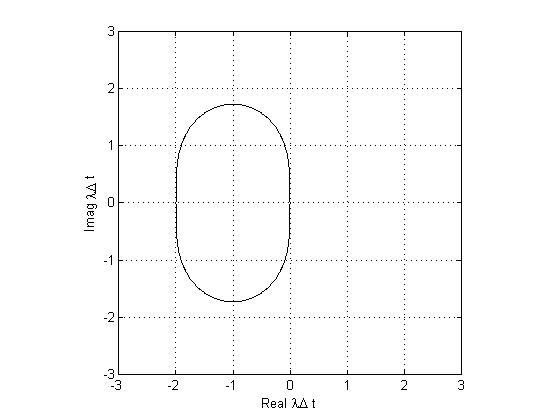
\includegraphics[width=\textwidth]{rk2.jpg}
                \caption{RK 2}
	\end{subfigure}
	\begin{subfigure}[b]{0.4\textwidth}
		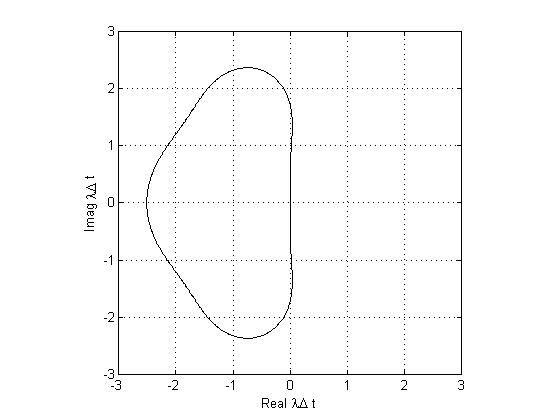
\includegraphics[width=\textwidth]{rk3.jpg}
                \caption{RK 3}
	\end{subfigure}
	\begin{subfigure}[b]{0.4\textwidth}
		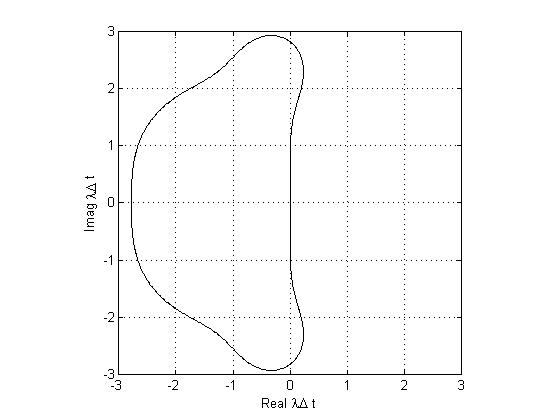
\includegraphics[width=\textwidth]{rk4.jpg}
                \caption{RK 4}
	\end{subfigure}
	\caption{Region of Stability for Range Kutta Method}
	\label{regofstab}
\end{figure}
Any differential equation which after discretization has the value of $\lambda \Delta t$ lying inside this bounded region would result in a stable solution using Runge Kutta Order 2 method. Moving ahead with \textbf{RK 3}, the amplification factor can be obtained as shown below
\begin{eqnarray}
y_{i+1} =& y_i + \frac{1}{6}h(k_1 + 4k_2 + k_3)
=& y_i + \frac{h}{6}(\lambda y_i +4\lambda(y_i+\frac{h\lambda y_i}{2})+\lambda (y_i -\lambda hy_j+2h\lambda(y_i+\frac{h\lambda y_i}{2}))) \nonumber \\
=& y_i + h\lambda y_i + \frac{(h\lambda)^2}{2} + \frac{(h\lambda)^3}{6} \nonumber \\
\Rightarrow =& g(z) = 1 + z + \frac{z^2}{2}+\frac{z^3}{6} \nonumber
\end{eqnarray}
while for \textbf{RK 4} the expressions can be similarly obtained to be as shown below:
\[ g(z) = 1 + z+ \frac{z^2}{2}+\frac{z^3}{6} + \frac{z^4}{24} \] 
Going through all the expressions one can easily see how with each order an extra term gets added which is basically expanding $u^{\prime}(t)$ and truncating the extension depending on the order of accuracy needed. This also verifies the basis of Runge Kutta methods. Region of eigen stability plots obtained are showcased in Figure \ref{regofstab}. Thus for an ODE to be solved using Runge Kutta methods, the value of $\lambda \Delta t$ should lie in the bounded regions which depends on the order of accuracy required.
\section{ROS: Both space \& time}
Now we already have the ROS for RK methods of all the requisite orders. Hence next we are trying to look how well does it work on the wave equation. We are now going to look into both the discretizations together. The wave equation has a first order differential operator for both space and time. Discretizing the space operator:
\[\frac{\partial u}{\partial t}= -a\frac{(u_{j+1}(t)-u_{j-1}()t)}{2h}\]
As we know the MOL needs a well defined cauchy problem with boundary conditions. So here we need the boundary conditions also. Using periodic boundary condition $u(0,t) = u(L,t)$, the problem becomes well posed and all the corresponding equations can now be written. Implementing the \textbf{RK 2} on the above equation and solving we get:
\begin{eqnarray}
u^{n+1}_{j}=&u^{n}_{j} -\frac{ak}{4h}(u^{*}_{j+1} -u^{*}_{j-1}) \nonumber \\
=& u^{n}_{j} - \frac{ak}{4h}u^{n}_{j+1}+(\frac{ak}{4h})^2(u^{n}_{j+2}-u^{n}_{j})+\frac{ak}{4h}-(\frac{ak}{4h})^2(u^{n}_{j}-u^{n}{j-2}) \nonumber \\
\end{eqnarray}
Converting this equation into differential form with $u^{\prime}_{j}(t)$ defined as that for Euler form $\frac{u^{n+1}_{j}-u^{n}_{j}}{k}$:
\[u^{\prime}_{j} = -\frac{a}{4h}(u^{n}_{j+1}-u^{n}_{j-1}) +k(\frac{a}{4h})^2(u^{n}_{j+2}+u^{n}_{j-2}-2u^{n}_{j})\]
All the corresponding equations including the boundary can be described as:
\begin{eqnarray}
u^{\prime}_{1} &=&  -\frac{a}{4h}(u^{n}_{2} - u^{n}_{m+1})+k(\frac{a}{4h})^2(u^{n}_{3}-2u^{n}_{1}+u^{n}_{m}) \nonumber \\
u^{\prime}_{2} &=&  -\frac{a}{4h}(u^{n}_{3} - u^{n}_{1})+k(\frac{a}{4h})^2(u^{n}_{4}-2u^{n}_{2}+u^{n}_{m+1}) \nonumber \\
for\ j\in[3,m-1] \nonumber \\
u^{\prime}_{j} &=& -\frac{a}{4h}(u^{n}_{j+1}-u^{n}_{j-1}) +k(\frac{a}{4h})^2(u^{n}_{j+2}+u^{n}_{j-2}-2u^{n}_{j}) \nonumber \\
u^{\prime}_{m} &=&  -\frac{a}{4h}(u^{n}_{m+1} - u^{n}_{m-1})+k(\frac{a}{4h})^2(u^{n}_{1}-2u^{n}_{m}+u^{n}_{m-2}) \nonumber \\
u^{\prime}_{m+1} &=&  -\frac{a}{4h}(u^{n}_{1} - u^{n}_{m})+k(\frac{a}{4h})^2(u^{n}_{2}-2u^{n}_{m+1}+u^{n}_{m-1}) \nonumber
\end{eqnarray}
This system of equations can be easily represented by the differential equation form given by:
$$\mathbf{U^{\prime}}(t) = \mathbf{AU}(t)$$ 
where 
\[ 
\mathbf{U}(t) = \begin{pmatrix}
u_{1}(t) \\ u_{2}(t) \\ \ldots \\ u_{m+1} \\
\end{pmatrix}
\ , \
\mathbf{U^{\prime}}(t) = \begin{pmatrix}
u^{\prime}_{1}(t) \\ u^{\prime}_{2}(t) \\ \ldots \\ u^{\prime}_{m+1} \\
\end{pmatrix}
\]
and
\[
\mathbf{A} = 
\frac{-a}{4h}
\begin{pmatrix}
0 & 1 & 0 & \ldots & 0 & -1 \\
-1& 0 & 1 & \ldots & 0 &  0 \\
0 & -1& 0 & \ldots & 0 &  0 \\
\vdots & \vdots & \vdots & \ddots & \vdots & \vdots \\ 
1 & 0 & 0 & \ldots & -1 & 0 \\
\end{pmatrix}
+\frac{a^2 k}{(4h)^2}
\begin{pmatrix}
-2& 0 & 1 & 0 & \ldots & 1 & 0 \\
0 &-2 & 0 & 1 & \ldots & 0 & 1 \\
1 & 0 &-2 & 0 & \ldots & 0 & 0 \\
\vdots & \vdots & \vdots & \vdots & \ddots & \vdots & \vdots \\
0 & 1 & 0 & 0 & \ldots & 0 & -2 \\
\end{pmatrix}
\]
Writing the two comprising matrix as $A_1$ and $A_2$
\[\mathbf{A} = \frac{-a}{4h} \mathbf{A_1} +\frac{a^2 k}{(4h)^2} \mathbf{A_2}\]
Since we have two matrices here, lets discuss them seperately. We are going to look into their properties which can help us estimate their eigen values since its their eigen values will help us determine the ROS.  \newline
\begin{itemize}
\item Matrix $A_1$ can be easily observed to be skew symmetric following the property $A_1^T = - A_1$. Now for a skew symmeteric matrix of order (m+1), there exist $\frac{(m+1)}{2}$ pairs of eigen values given $m+1$ is even or $\frac{m}{2}$ pairs and zero given $m+1$ is odd. The eigen values are also imaginary since all the elements of the matrix are real. The eigen values for this matrix are given by:
$$\beta_{p} = -2i \sin (2\pi ph),\ 	for\ p=1,\ 2,.....,m+1$$
\item Matrix $A_2$ is symmetric as it follows $A_2^T = A_2$. All the entries being real, this matrix has real eigen values. For m=4, the eigen values are $0, \pm3.618$ and $\pm1.382$, for m=5 the eigen values are 0 and -3 and for m=7, the eigen values are 0,-2 and -4. Let these values be $\alpha_i$.
\end{itemize}
Now the eigen values of the system can be written as:
$$\lambda_i = \alpha_i\frac{a^2}{(4h)^2}+i\frac{a}{2h}\sin(2\pi ph)$$
As the eigen values either lie on the left hand side of the argand plane and completely inside the region of Runge Kutta methods, hence these methods can be verified as \textbf{stable} for ak/2h < 1.\\
A similar analysis can also be done for the Upwind Scheme. In this case the matrix is assymetric. Hence one cannot directly predict their eigen values. For example, in case of Upwind scheme with RK 3, the matrix obtained is:
\[U^{\prime}=\frac{-a}{h} A_1 + \frac{a^2 k}{h^2} A_2\]
where $A_1$ and $A_2$ are defined as below:
\[
\mathbf{A_1} = 
\begin{pmatrix}
1 & 0 & 0 & \ldots & 0 & -1 \\
-1& 1 & 0 & \ldots & 0 &  0 \\
0 & -1& 1 & \ldots & 0 &  0 \\
\vdots & \vdots & \vdots & \ddots & \vdots & \vdots \\ 
0 & 0 & 0 & \ldots & -1 & 1 \\
\end{pmatrix}
\mathbf{A_2} = 
\begin{pmatrix}
1 & 0 & 1 & 0 & \ldots & 1 & -2 \\
-2& 1 & 0 & 0 & \ldots & 0 & 1 \\
1 &-2 & 1 & 0 & \ldots & 0 & 0 \\
\vdots & \vdots & \vdots & \vdots & \ddots & \vdots & \vdots \\
0 & 0 & 0 & 0 & \ldots &-2 & -1 \\
\end{pmatrix}
\]
For a 6x6 matrix, $A_1$ has eigen values 0, 0.5+0.866i, 0.5-0.866i, 1.5+1.866i, 1.5-0.866i and 2 while that for $A_2$ are 5, -1+1.732i, -1-1.732i,1+1.732i,1-1.732i and 1. Clearly 5+0=5 will never lie in the left half plane and hence it will not be inside the ROS for RK3. Thus we can directly say that this method is unstable. Due to difficulty in determining the eigen values of a general (m+1)x(m+1) matrix, we have only touched a simple example. For further analysis lets look into the next section which would through further light on stability analysis of these schemes.
\chapter{Analysis}
\section{Central Difference in space}
An easy way to reduce the error is to approximate the differential operator using central difference approximation.However it should be kept in mind that Central Difference approximation involves using the neighbouring elements to estimate the value of the cell in question which in turn increases the spatial dependency hence requiring greater information. Its order of accuracy is $O(\Delta x^2)$.
\subsection{Range Kutta order 2}
Range Kutta of order two are a family of methods in itself. This is because having enforced the error, a set of parametric equations is obtained in a variable alpha($\alpha$). Depending on the value of $\alpha$ many methods have been standardized like Heun's method $\alpha=\frac{1}{2}$, mid-point method $\alpha=1$, Ralston's method $\alpha=\frac{2}{3}$. Here we would be using the Mid-point method.
Given the equation
\[\frac{\partial u(x,t)}{\partial t}+c\frac{\partial u(x,t)}{\partial x} = 0 \]
Discretizing the equation using the RK2-central difference scheme:
\begin{eqnarray}
u^{n+1}_{i} = u^{n}_{i} - c\Delta t k_2 \label{ctdeqn}\\ 
where \nonumber \\
k_1 &=& \frac{u_{i+1}^{n} -u_{i-1}^{n}}{2\Delta x} \nonumber \\
k_2 &=& \frac{u_{i+1}^{n+\frac{1}{2}} -u_{i-1}^{n+\frac{1}{2}}}{2\Delta x} \nonumber
\end{eqnarray}
Here the values at half time step is evaluated using euler approximation with slope $k_1$ as illustrated by the following expression:
\[u_{i}^{n+\frac{1}{2}} = u_{i}^{n} - \frac{c\Delta t}{\Delta x}k_1 \]
The next step is using the fourier term $\xi^{n}e^{j\chi i}$ for $u^{n}_{i}$ in the discretized equation where $j$ stands for $\sqrt{-1}$
\begin{eqnarray}
\xi^{n+1}e^{j\chi i} &=& \xi^{n}e^{j\chi i} -\frac{c\Delta t}{2\Delta x}(\xi^{n+\frac{1}{2}}(e^{j\chi(i+1)}-e^{j\chi(i-1)}) \label{eqn}\\
\xi&=& 1 -\frac{c\Delta t}{2\Delta x}(\xi^{\frac{1}{2}}(e^{j\chi}-e^{j\chi(-1)}) \nonumber
\end{eqnarray}
Let $d=\frac{c\Delta t}{\Delta x}$. The equation (\ref{eqn}) now becomes:
\begin{eqnarray}
\xi + d \xi^{\frac{1}{2}}\frac{(\cos{\chi}+j\sin{\chi} - \cos{-\chi}+j\sin{-\chi})}{2} &=& 1 \nonumber \\
\xi + d \xi^{\frac{1}{2}}\frac{(\cos{\chi}+j\sin{\chi}) - (\cos{\chi}-j\sin{\chi})}{2} &=& 1 \nonumber \\
\xi + d \xi^{\frac{1}{2}}\frac{(\cos{\chi}+j\sin{\chi} - \cos{\chi}+j\sin{\chi})}{2}&=&1\nonumber \\
\xi + d \xi^{\frac{1}{2}}\frac{2j\sin{\chi}}{2}-1&=&0
\end{eqnarray}
This is a quadratic equation in $G := \sqrt{\xi}$. Product of the roots is -1. \newline
$G_1G_2 = -1$ or $|G_1||G_2| = 1$
Hence there arise two posibilities mentioned here under:
\begin{enumerate}
\item $|G_1|=|G_2|=1$ in which case there is no gain and the solution would not converge.
\item $|G_1|<1$ and $|G_2|> 1$ or $|G_1|<1$ and $|G_2|> 1$. In either case it is evident that one of the gain factor would exceed 1. Hence the equation would not converge to a solution once again.
\end{enumerate}
Hence it can be concluded from Von-Neumann Analysis that this scheme is \textbf{unconditionally unstable}. 
\subsection{Range Kutta order 3}
Discretization of the equation would be:
\begin{eqnarray}
u^{n+1}_{i} &=& u^{n}_{i} - c\Delta t \frac{(k_1+4k_2+k_3)}{6}
\\with \nonumber\\
k_1 &=& \frac{u_{i+1}^{n} -u_{i-1}^{n}}{2\Delta x} \nonumber \\
k_2 &=& \frac{u_{i+1}^{n+\frac{1}{2}} -u_{i-1}^{n+\frac{1}{2}}}{2\Delta x} \nonumber\\
k_3 &=& \frac{u_{i+1}^{n+1} -u_{i-1}^{n+1}}{2\Delta x} \nonumber
\end{eqnarray}
where $u_{i+1}^{n+\frac{1}{2}}$ and $u_{i+1}^{n+1}$ are evaluated by linear approximation using $u^{n}_{i}$ with a step of $\Delta t/2$ and $\Delta t$ using slope $k_1$ and $2k_2-k_1$ respectively.
Substituting $\xi^{n}e^{j\chi i}$ into the equation we get the following equation in $\xi$
\begin{eqnarray}
\xi &=& 1-2dj\sin{\chi}\frac{1+4\xi^{\frac{1}{2}}+\xi}{12} \nonumber \\
which\ can\ be\ rearranged\ into \nonumber \\
0 &=& A\xi+B\xi^{\frac{1}{2}} + C \label{quadratic}\\
with\ A &=& \frac{d}{6}j\sin{\chi} + 1 \nonumber\\
B &=& \frac{4d}{6}j\sin{\chi} \nonumber\\
C &=& \frac{d}{6}j\sin{\chi} - 1 \nonumber
\end{eqnarray}
Evaluating $D = B^2 - AC$ we get $D = 1-\frac{d^2{\sin^2{\chi}}}{3}$
Thus the root of equation (\ref{quadratic}) are found to be as follows:
\begin{eqnarray}
|G_i|^2 := |\xi^\frac{1}{2}|^2 &=& |\frac{\frac{-4}{6}dj\sin{\chi}\pm \sqrt{D}}{2(\frac{1}{6}dj\sin{\chi}+1)}|^2 \nonumber\\
&=& \frac{\frac{4}{36}d^2\sin^2{\chi}+4}{4(\frac{1}{36}d^2\sin^2{\chi}+1)}\label{root}\\
&=& 1
\end{eqnarray}
Now if amplification factor remains as 1, convergence would not occur and therefore it can be concluded that this scheme is \textbf{unstable}. It can also be verified for a range of values using the code given below.  
\begin{lstlisting}
N = 21;
chi = linspace(-1,1,N);
j = sqrt(-1);
d = linspace(-2,2,N);
D = ones(N,N);
rxi = ones(N,N);
for m = 1:N
    for n = 1:N
        D(m,n) = (2/3*d(n)*j*chi(m))^2-4*((d(n)*j*chi(m)/6)^2-1);
        rxi(m,n) = (-2/3*d(n)*j*chi(m) - sqrt(D(m,n)))/(2*(1+d(n)*j*chi(m)/6));
        rxi(m,n) = rxi(m,n)^2;
    end
end
rximag = (abs(rxi));
\end{lstlisting}
After running the code, it is observed that the value of variable rximag is fixed at one for every $\chi$ and d;
\subsection{Range Kutta order 4}
Discretization for RK4 with central difference approximation would be as shown here:
\begin{eqnarray}
u^{n+1}_{i} &=& u^{n}_{i} - c\Delta t \frac{(k_1+2k_2+2k_3+k_4)}{6}
\\with \nonumber\\
k_1 &=& \frac{u_{i+1}^{n} -u_{i-1}^{n}}{2\Delta x} \nonumber \\
k_2 &=& \frac{u_{i+1}^{n+\frac{1}{2}} -u_{i-1}^{n+\frac{1}{2}}}{2\Delta x} \label{k2}\\
k_3 &=& \frac{u_{i+1}^{n+\frac{1}{2}} -u_{i-1}^{n+\frac{1}{2}}}{2\Delta x} \label{k3}\\
k_4 &=& \frac{u_{i+1}^{n+1} -u_{i-1}^{n+1}}{2\Delta x} \nonumber
\end{eqnarray}
where $u_{i+1}^{n+\frac{1}{2}}$ in equation (\ref{k2}) and (\ref{k3}) are evaluated by linear approximation using $u^{n}_{i}$ with a step of $\Delta t/2$ using slope $k_1$ and $2k_2$ while $u_{i+1}^{n+1}$ is linearly approximated from $u^{n}_{i}$ with half time step and slope $k_3$. \\
Substituting $\xi^{n}e^{j\chi i}$ into the equation we get the following equation in $\xi$ \\
\begin{eqnarray}
\xi &=& 1-2dj\sin{\chi}\frac{1+2\xi^{\frac{1}{2}}+2\xi^{\frac{1}{2}}+\xi}{12} \nonumber \\
\xi &=& 1-2dj\sin{\chi}\frac{1+4\xi^{\frac{1}{2}}+\xi}{12} \label{samequadratic}
\end{eqnarray}
Equation (\ref{samequadratic}) is exactly the same quadratic equation as obtained while doing the Von Neumann analysis of RK3 with central difference [refer equation (\ref{quadratic}).
Therefore it can be concluded that this scheme is also \textbf{unconditionally stable}.
\newpage
\section{Upwind Scheme in Space}
Based on direction of velocity, spatial discretization is varied. The truncation error in this scheme is much higher than what is observed for Central Difference. Thus deviation may occur.
\subsection{Range Kutta order 2}
Using RK2 time integration and discretizing the equation using the scheme (midpoint method $\alpha = \frac{1}{2}$):
\[u^{n+1}_{i} = u^{n}_{i} - c\Delta t k_2\]
where for $c>0$
\begin{eqnarray}
k_1 &=& \frac{u_{i}^{n} -u_{i-1}^{n}}{2\Delta x} \nonumber \\
k_2 &=& \frac{u_{i}^{n+\frac{1}{2}} -u_{i-1}^{n+\frac{1}{2}}}{2\Delta x} \nonumber
\end{eqnarray}
and for $c<0$
\begin{eqnarray}
k_1 &=& \frac{u_{i+1}^{n} -u_{i}^{n}}{2\Delta x} \nonumber \\
k_2 &=& \frac{u_{i+1}^{n+\frac{1}{2}} -u_{i}^{n+\frac{1}{2}}}{2\Delta x} \nonumber
\end{eqnarray}
Here the values at half time step is evaluated in the same manner as done while solving for Central Difference Scheme.
\[u_{i}^{n+\frac{1}{2}} = u_{i}^{n} - \frac{c\Delta t}{\Delta x}k_1 \]
Putting in the fourier term $\xi^{n}e^{j\chi i}$ for $u^{n}_{i}$ in the discretized equation.
\begin{eqnarray}
for\ c>0\\
\xi^{n+1}e^{j\chi i} &=& \xi^{n}e^{j\chi i} -\frac{c\Delta t}{\Delta x}(\xi^{n+\frac{1}{2}}(e^{j\chi(i)}-e^{j\chi(i-1)})) \\
\Rightarrow \xi&=& 1 -\frac{c\Delta t}{\Delta x}(\xi^{\frac{1}{2}}(1-e^{j\chi(-1)}) \nonumber \label{posC} \\
for\ c<0\\
\xi^{n+1}e^{j\chi i} &=& \xi^{n}e^{j\chi i} -\frac{c\Delta t}{\Delta x}(\xi^{n+\frac{1}{2}}(e^{j\chi(i+1)}-e^{j\chi(i)})) \\
\Rightarrow\xi&=& 1 -\frac{c\Delta t}{\Delta x}(\xi^{\frac{1}{2}}(e^{j\chi}-1)) \nonumber\label{negC} \\
\end{eqnarray}
Here c has been considered with sign. Let $d=\frac{c\Delta t}{\Delta x}$. Now equation (\ref{posC}) and (\ref{negC}) takes the form of a quadratic equation:
\begin{eqnarray*}
A\xi + B\sqrt{\xi} + C &=&0 \\
with\ A &=& 1 \\
for\  d>0 \\ B &=& |d|(1-e^{-j\chi}) \\
for\  d<0 \\B &=& -|d|(e^{j\chi} -1) \\
C &=& -1
\end{eqnarray*}
This is a quadratic equation in $G := \sqrt{\xi}$. Product of the roots is -1. \newline
$G_1G_2 = -1$ or $|G_1||G_2| = 1$
With respect to their magnitude, again the same two cases arise :
\begin{enumerate}
\item $|G_1|=|G_2|=1$
\item $|G_1|<1$ and $|G_2|> 1$ or $|G_1|<1$ and $|G_2|> 1$. 
\end{enumerate}
In either case it is evident that one of the gain factor would exceed 1. Using the same arguement as used while evaluating central differnce scheme with RK2, it can be concluded that this scheme is found to be \textbf{unconditionally unstable} through Von-Neumann analysis.
\subsection{Range Kutta order 3}
Discretization of the equation would be:
\begin{eqnarray}
u^{n+1}_{i} &=& u^{n}_{i} - c\Delta t \frac{(k_1+4k_2+k_3)}{6} \nonumber
with\ for\ c>0 \nonumber\\
k_1 &=& \frac{u_{i}^{n} -u_{i-1}^{n}}{2\Delta x} \nonumber \\
k_2 &=& \frac{u_{i}^{n+\frac{1}{2}} -u_{i-1}^{n+\frac{1}{2}}}{2\Delta x} \nonumber\\
k_3 &=& \frac{u_{i}^{n+1} -u_{i-1}^{n+1}}{2\Delta x} \nonumber
\end{eqnarray}
\begin{eqnarray}
for\ c<0 \nonumber\\
k_1 &=& \frac{u_{i+1}^{n} -u_{i}^{n}}{2\Delta x} \nonumber \\
k_2 &=& \frac{u_{i+1}^{n+\frac{1}{2}} -u_{i}^{n+\frac{1}{2}}}{2\Delta x} \nonumber\\
k_3 &=& \frac{u_{i+1}^{n+1} -u_{i}^{n+1}}{2\Delta x} \nonumber
\end{eqnarray}
where $u_{i+1}^{n+\frac{1}{2}}$ and $u_{i+1}^{n+1}$ are evaluated by linear approximation using $u^{n}_{i}$ with a step of $\Delta t/2$ and $\Delta t$ using slope $k_1$ and $2k_2-k_1$ respectively. Also here c has been considered with sign for appropriate direction.
Substituting $\xi^{n}e^{j\chi i}$ into the equation we get the following equation in $\xi$\\
\begin{eqnarray}
\xi &=& 1- \frac{1}{6}(1-e^{-j\chi}(1+4\xi^\frac{1}{2} +\xi)\nonumber \\
Rearranging\ into\ a\ quadratic \nonumber \\
0 &=& A\xi+B\xi^{\frac{1}{2}} + C \label{uprk3}\\
where\ for\ c>0 \nonumber\\
A &=& \frac{1}{6}d(1-e^{-j\chi})+1  \nonumber\\
B &=& \frac{4}{6}d(1-e^{-j\chi}) \nonumber\\
C &=& \frac{1}{6}d(1-e^{-j\chi}) - 1 \nonumber
and\ for\ c<0 \nonumber\\
A &=& \frac{1}{6}d(e^{j\chi}+1)+1  \nonumber\\
B &=& \frac{4}{6}d(e^{-j\chi}+1) \nonumber\\
C &=& \frac{1}{6}d(e^{-j\chi}+1) - 1 \nonumber
\end{eqnarray}
Evaluating the value of discriminant $D = B^2 - AC$ we get $D_1 = 4 + \frac{12}{36}d^2(1-e^{-j\chi})^2$ when $c>0$
and $D_2 = 4 + \frac{12}{36}d^2(e^{j\chi}+1)^2$ when $c<0$.
But this itself is a complex number. 
 \begin{eqnarray}
|G_i|^2 := |\xi^\frac{1}{2}|^2 &=& |\frac{\frac{-4}{6}d(1-e^{-j\chi})\pm \sqrt{D}}{2(\frac{1}{6}d\sin{\chi}+1)}|^2 \label{uprk3root}\\
\end{eqnarray}
Equation (\ref{uprk3root}) could not be evaluated properly for the magnitude of root. To evaluate how does the roots behave, MATLAB code was written and the magnitude of both the roots was checked for a wide range of values. The code is provided below. The results demonstrated that the two roots never agreed to be less than one for any values of $\chi$ or d. This demonstrates that this scheme like RK 2 with upwind is \textbf{unstable}.
\begin{lstlisting}
N = 11;
chi = linspace(-50,50,N);
j = sqrt(-1);
d = linspace(0,5,N);
D = ones(N,N);
rxi1 = ones(N,N);
rxi2 = ones(N,N);
for m = 1:N
    xp = (1-exp(-j*chi(m)));
    for n = 1:N       
        D(m,n) = (2*d(n)/3*xp)^2-4*((d(n)*xp/6)^2-1);
        rxi1(m,n) = (-2*d(n)/3*xp+sqrt(D(m,n)))/(2*d(n)/6*xp - 2);
        rxi1(m,n) = rxi1(m,n)^2;
        rxi2(m,n) = (-2*d(n)/3*xp-sqrt(D(m,n)))/(2*d(n)/6*xp - 2);
        rxi2(m,n) = rxi2(m,n)^2;
    end
end
rximag1 = (abs(rxi1));
rximag2 = (abs(rxi2));
\end{lstlisting}
\subsection{Range Kutta order 4}
Discretization for RK4 with central difference approximation would be as shown here:
\begin{eqnarray}
u^{n+1}_{i} &=& u^{n}_{i} - c\Delta t \frac{(k_1+2k_2+2k_3+k_4)}{6}
\\with\ for\ c>0 \nonumber\\
k_1 &=& \frac{u_{i}^{n} -u_{i-1}^{n}}{2\Delta x} \nonumber \\
k_2 &=& \frac{u_{i}^{n+\frac{1}{2}} -u_{i-1}^{n+\frac{1}{2}}}{2\Delta x} \label{rk4k2a}\\
k_3 &=& \frac{u_{i}^{n+\frac{1}{2}} -u_{i-1}^{n+\frac{1}{2}}}{2\Delta x} \label{rk4k3a}\\
k_4 &=& \frac{u_{i}^{n+1} -u_{i-1}^{n+1}}{2\Delta x} \nonumber
\end{eqnarray}
\begin{eqnarray}
for\ c<0 \nonumber \\
k_1 &=& \frac{u_{i+1}^{n} -u_{i}^{n}}{2\Delta x} \nonumber \\
k_2 &=& \frac{u_{i+1}^{n+\frac{1}{2}} -u_{i}^{n+\frac{1}{2}}}{2\Delta x} \label{rk4k2b}\\
k_3 &=& \frac{u_{i+1}^{n+\frac{1}{2}} -u_{i}^{n+\frac{1}{2}}}{2\Delta x} \label{rk4k3b}\\
k_4 &=& \frac{u_{i+1}^{n+1} -u_{i}^{n+1}}{2\Delta x} \nonumber
\end{eqnarray}
where $u_{i+1}^{n+\frac{1}{2}}$ in equation (\ref{rk4k2a})/(\ref{rk4k3a}) and (\ref{rk4k2b})/(\ref{rk4k3b}) are evaluated by linear approximation mentioned before.
Substituting $\xi^{n}e^{j\chi i}$ into the equation we get the following equation in $\xi$
\begin{eqnarray}
\xi &=& 1- \frac{1}{6}(1-e^{-j\chi}(1+2\xi^\frac{1}{2}+2\xi^\frac{1}{2} +\xi)\nonumber \\
Rearranging\ into\ a\ quadratic \nonumber \\
0 &=& A\xi+B\xi^{\frac{1}{2}} + C \label{uprk4}\\
where\ for\ c>0 \nonumber\\
A &=& \frac{1}{6}d(1-e^{-j\chi})+1  \nonumber\\
B &=& \frac{4}{6}d(1-e^{-j\chi}) \nonumber\\
C &=& \frac{1}{6}d(1-e^{-j\chi}) - 1 \nonumber \\
and\ for\ c<0 \nonumber\\
A &=& \frac{1}{6}d(e^{j\chi}+1)+1  \nonumber\\
B &=& \frac{4}{6}d(e^{-j\chi}+1) \nonumber\\
C &=& \frac{1}{6}d(e^{-j\chi}+1) - 1 \nonumber
\end{eqnarray}
The quadratic equation (\ref{uprk4}) is the same as obtained before incase of RK3 with upwind scheme equation (\ref{uprk3}). And hence one can again say that this scheme stands to be \textbf{unstable} as well.
\newpage
\chapter{Results}
\section{Stability Analysis}
Von Neumann Stability analysis provides an idea of how efficient a particular method is in solving the 1-d wave equation and whether the solution would numerically converge or not. For a better understanding, these methods were coded and all the six cases were plotted.The graphs are as shown below.
\begin{figure} [h]
	\centering
	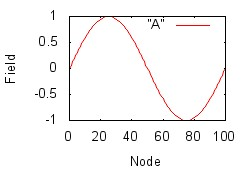
\includegraphics{Actual.jpeg}  
	\caption{Initial pulse} 
	\label{fig:initial} 
\end{figure} 
\begin{figure}[h!]  
	\centering
	\begin{subfigure}[b]{0.4\textwidth}
		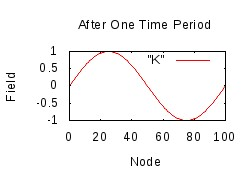
\includegraphics[width=\textwidth]{rk2ctd.jpeg}
                \caption{RK 2}
                \label{fig:rk2ctd}
	\end{subfigure}
	\begin{subfigure}[b]{0.4\textwidth}
		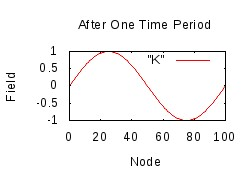
\includegraphics[width=\textwidth]{rk3ctd.jpeg}
                \caption{RK 3}
                \label{fig:rk3ctd}
	\end{subfigure}
	\begin{subfigure}[b]{0.4\textwidth}
		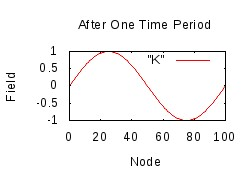
\includegraphics[width=\textwidth]{rk3ctd.jpeg}
                \caption{RK 4}
                \label{fig:rk4ctd}
	\end{subfigure}
	\caption{RK in time and Central in space}
	\label{Central}
\end{figure}
Figure \ref{fig:initial} is how the pulse appears initially. Its a sinusoid travelling at a speed of 0.5 m/s having a wavelength is 1 m. The complete domain has been divided into 100 segments and time march is of 0.001 s. Figure \ref{Central} demonstrates the results obtained by using central difference approximation for spatial coordinate while RK time integrators of order 2, 3 and 4 have been employed. The results are very much similar. This can be attributed to more sensitivity towards spatial discretization rather than time discretization. 
\begin{figure}[h]  
	\centering
	\begin{subfigure}[b]{0.4\textwidth}
		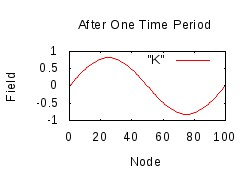
\includegraphics[width=\textwidth]{rk2upw.jpeg}
                \caption{RK 2}
                \label{fig:rk2upw}
	\end{subfigure}
	\begin{subfigure}[b]{0.4\textwidth}
		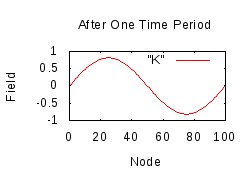
\includegraphics[width=\textwidth]{rk3upw.jpeg}
                \caption{RK 3}
                \label{fig:rk3upw}
	\end{subfigure}
	\begin{subfigure}[b]{0.4\textwidth}
		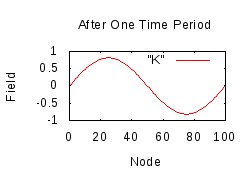
\includegraphics[width=\textwidth]{rk3upw.jpeg}
                \caption{RK 4}
                \label{fig:rk4upw}
	\end{subfigure}
	\caption{RK in time and Upwind in space}
	\label{Upwind}
\end{figure}
The plots shown above (\ref{Upwind}) demonstrate the unstability of this scheme as opposed to central difference. Moreover, upwind is a dispersive scheme. It relies on $\Delta x\ and\ \Delta t$ for convergence. If these two parameters are fairly high then its implication is appearance of some undampened components which travel at a speed different than that of a wave. 
\section{Error analysis}
Table \ref{normtab} lists the values of error norms obtained by comparing the full sine pulse after one time period with the actual solution. Figure \ref{Normscd} illustrates the error norms for the central difference scheme while figure \ref{Normsupw} shows the norms for upwind scheme. Upwind scheme being unstable undergoes an increase in error as the time proceeds. This is supported by higher values of error for Upwind scheme depicted in the table \ref{normtab}. Within the RK schemes, RK4 should definitely yield lower error values which is apparent form the $||L||_{\infty}$. But the values are very close to each other even at the point of difference.\\
Another striking property that one finds here is that the 1-d wave equation is not very responsive to the order of time stepping as compared to spatial stepping. For example for a grid of 100 points in space seperated by 0.01m each are subjected to a wave travelling at 0.001m/s should same error results of 0.760332, 0.839371 and 1.1817 for $L_1$,$L_2$ and $L_{\infty}$ respectively for both RK2 and RK4 solvers. This may be due to the dependence of the difference equation on Courant number. It is observed that the solution does not converge for higher courant numbers. Going by the symmetricity of the governing equation, the courant number decides the dominance. As it's value is lower than 1, the dominant error is the spatial one. 
\begin{figure}[h!]  
	\centering
	\begin{subfigure}[b]{0.7\textwidth}
		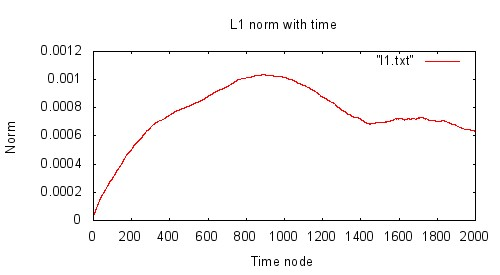
\includegraphics[width=\textwidth]{l1.jpeg}
                \caption{$||L||_1$ norm}
                \label{fig:l1}
	\end{subfigure}
	\begin{subfigure}[b]{0.7\textwidth}
		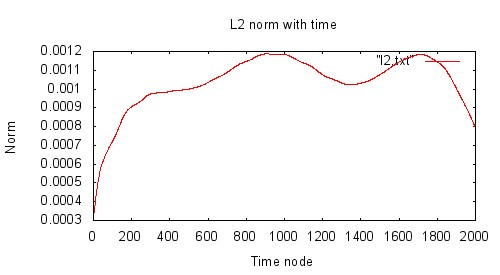
\includegraphics[width=\textwidth]{l2.jpeg}
                \caption{$||L||_2$ norm}
                \label{fig:l2}
	\end{subfigure}
	\begin{subfigure}[b]{0.7\textwidth}
		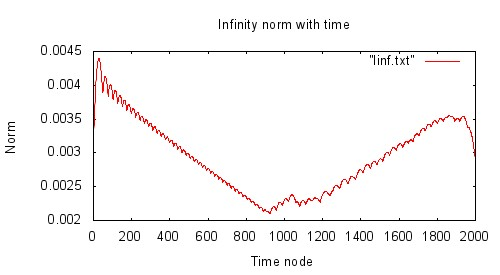
\includegraphics[width=\textwidth]{linf.jpeg}
                \caption{$||L||_{\infty}$ norm}
                \label{fig:linf}
	\end{subfigure}
	\caption{Plot of norm versus nodes for Central Difference}
	\label{Normscd}
\end{figure}
\begin{figure}[h!]  
	\centering
	\begin{subfigure}[b]{0.7\textwidth}
		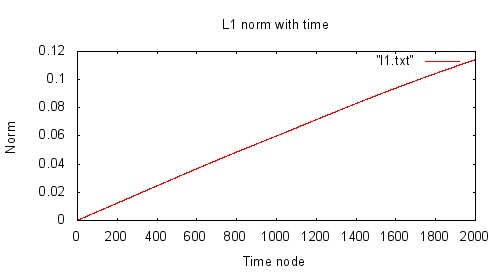
\includegraphics[width=\textwidth]{upwl1.jpeg}
                \caption{$||L||_1$ norm}
                \label{fig:upwl1}
	\end{subfigure}
	\begin{subfigure}[b]{0.7\textwidth}
		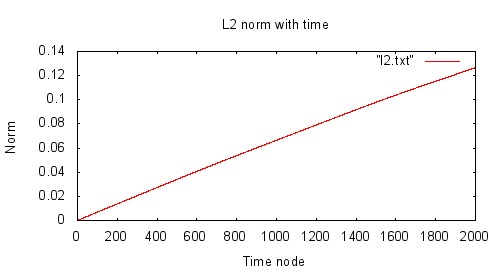
\includegraphics[width=\textwidth]{upwl2.jpeg}
                \caption{$||L||_2$ norm}
                \label{fig:upwl2}
	\end{subfigure}
	\begin{subfigure}[b]{0.7\textwidth}
		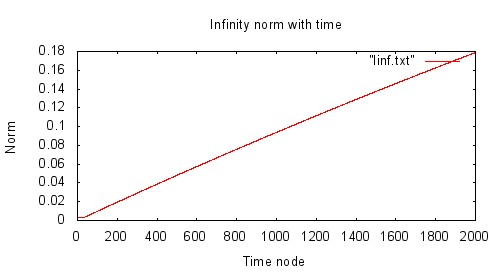
\includegraphics[width=\textwidth]{upwlinf.jpeg}
                \caption{$||L||_{\infty}$ norm}
                \label{fig:upwlinf}
	\end{subfigure}
	\caption{Plot of norm versus nodes for Upwind}
	\label{Normsupw}
\end{figure}
\begin{table}
\begin{center}
	\begin{tabular}{| l | l | l | l | l |}
	\hline
	\textbf{Space} & \textbf{Time} & \textbf{$L_1$ norm} & \textbf{$L_2$ norm} & \textbf{$L_{\infty}$ norm} \\ \hline
	Upwind & RK2 & 0.114110 & 0.126605 & 0.178862 \\ \hline
	Upwind & RK3 & 0.117532 & 0.130404 & 0.184232 \\ \hline
	Upwind & RK4 & 0.114110 & 0.126605 & 0.178861 \\ \hline
	Central Difference & RK2 & 0.00063504 & 0.000798315 & 0.0029159 \\ \hline
	Central Difference & RK3 & 0.00065957 & 0.000846769 & 0.0037232 \\ \hline
	Central Difference & RK4 & 0.00063946 & 0.000802771 & 0.0029164 \\ \hline
	\end{tabular}
\end{center}
\caption{Error Norm $\alpha=0.05$}
\label{normtab}
\end{table}
\section{Discussion}
\subsection{Diffusion}
Consider a half sinusoidal wave travelling at 0.5 m/s. With 0.001s as time step and the complete domain divided into grid points 0.01m apart RK methods were applied in conjunction with central difference and upwind schemes. Obtained solution after one time period (2000 time steps) was compared with the original wave [Figure \ref{disp}]. Since there wasn't much variation with respect to order of RK method employed, the redundant shapes have not been shown in the figure. It is clearly visible that the distortion has spread beyond the region it belongs to in both the cases. Infact, the distortion is more in case of Upwind scheme. Hence both the schemes in combination with RK method result in diffused wave. This is generally attributed to the damped waves that decay exponential\cite{it1}. For $d<1$ Fourier modes with some particular wavelength are not only damped but they also propagate at a higher phase velocity. Even further if try integrating the discretized equation, it won't be surprising to find some extra terms. Take for example the central difference with Runge Kutta order 2 (Eq. \ref{ctdeqn}) elaborated as under:
\begin{eqnarray}
u_{j}^{n+1} &=& u_{j}^{n} - \frac{c\Delta t}{2\Delta x}(u_{j+1}^{n+\frac{1}{2}} - u_{j-1}^{n+\frac{1}{2}}) \label{ctdrk2} \\
&=& u_{j}^{n} - \frac{c\Delta t}{2\Delta x}[u_{j+1}^{n}- \frac{c\Delta t}{2\Delta x}(u_{j+2}^{n}-u_{j}^{n}) - (u_{j-1}^{n}-\frac{c\Delta t}{2\Delta x}(u_{j}^{n}-u_{j-2}^{n}))] \nonumber \\
\Rightarrow u_{j}^{n+1}- u_{j}^{n} &=& - \frac{c\Delta t}{2\Delta x}(u_{j+1}^{n})-u_{j-1}^{n}) +(\frac{c\Delta t}{2\Delta x})^2[u_{j+2}^{n}-2u_{j}^{n}+u_{j-2}^{n}] \nonumber \\
\Rightarrow \frac{\partial u}{\partial t} &=& -c\frac{\partial u}{\partial x} + c^2\Delta t\frac{\partial^2 u}{\partial x^2} \label{xterm}
\end{eqnarray}
Looking at Eq \ref{xterm}, an extra term $\frac{c^2\Delta}{2} t\frac{\partial^2 u}{\partial x^2}$ is also being solved with the discretization we have opted for. This extra term reduces to zeros as $\Delta t \rightarrow 0$
\begin{figure}[h!]  
	\centering
	\begin{subfigure}[b]{0.4\textwidth}
		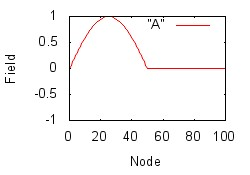
\includegraphics[width=\textwidth]{hfsine.jpeg}
                \caption{Initial Pulse}
                \label{fig:hfsine}
	\end{subfigure}
	\begin{subfigure}[b]{0.4\textwidth}
		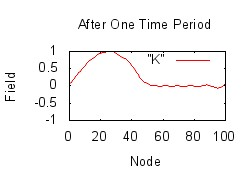
\includegraphics[width=\textwidth]{hfsinrk3ctd.jpeg}
                \caption{Central Difference}
                \label{fig:hfctd}
	\end{subfigure}
	\begin{subfigure}[b]{0.4\textwidth}
		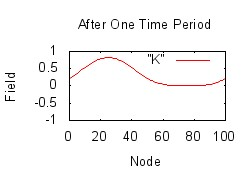
\includegraphics[width=\textwidth]{hfsinrk4upw.jpeg}
                \caption{Upwind}
                \label{fig:hfupw}
	\end{subfigure}
	\caption{Dispersion}
	\label{disp}
\end{figure}
\subsection{Case of a square wave}
Square waves are said to be comprised of infinitely many frequencies. This makes their case a little more interesting to study. We have seen the response of the Runge Kutta, Upwind and Central Difference to a pulse having only one frequency. Extending it further we had a glimpse of the results obtained for a half sine wave. Now let's look into the behaviour of these schemes for a square wave. The input square is as shown in Figure \ref{sqinit}.
\begin{figure}[h]
	\centering
	\begin{subfigure}[b]{0.5\textwidth}
		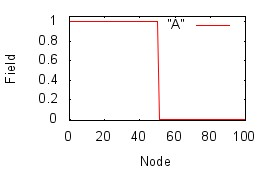
\includegraphics[width=\textwidth]{sqinit.jpeg}
                \caption{Square pulse}
                \label{sqinit}
	\end{subfigure}
	\begin{subfigure}[b]{0.5\textwidth}
		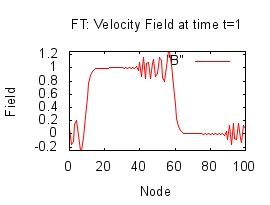
\includegraphics[width=\textwidth]{sqpulse2.jpeg}
                \caption{After 2 seconds}
                \label{sqpul2}
	\end{subfigure}
	\begin{subfigure}[b]{0.5\textwidth}
		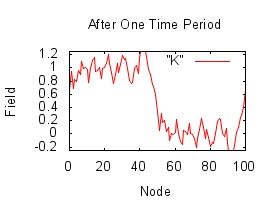
\includegraphics[width=\textwidth]{sqrk4ctd.jpeg}
                \caption{After 1 timeperiod}
                \label{sqctd}
	\end{subfigure}
\caption{Effect on a Square Pulse: RK4 and Central Difference}
\end{figure}
\\
Using RK 4 time integrator combined with central difference scheme for spatial coordinates, a lot of ripples are observed in the obtained wave. At the edges the amplitude of the ripples shoots up with the lowest amplitude just after that. This reminds us of the Fourier series  for a square wave. Such a square wave can be obtained with lesser error if large number of series terms are included. At the edges similar ripples exist in that case too. Wave propagation for a square wave numerically is very challenging anyways. At the point of seperation, the ripples are found to start first travelling down the pulse making the complete pulse comprise of many other small ripples as shown in Figure \ref{sqpul2}
\begin{thebibliography}{99}
\bibitem{it1}
MIT Open Course Ware. \emph{Finite Difference Discretization of Hyperbolic Equations Linear Problems}
Lectures 8 9 and 10
\bibitem{it2}
J.H.~Ferziger, M.~Peric. \emph{Computational Method for Fluid Dynamics}
Springer (third edition)
\bibitem{it3}
Advection FTCS lax and laxWendroff
\bibitem{it4}
Dr.~Johnson. \emph{Von Neumann Stability Analysis}
Lecture slides MATH65241, Semester 1-2008
\bibitem{it5}
Shasha~Xie, Dept~of~Applied~Mechanics,~Chalmers~University~of~Technology. \emph{Studies of Ercoftac Centrifugal Pump with OpenFOAM}
Master's Thesis
\bibitem{it6}
Steven.~C.~Chapra, Raymond~Canale. \emph{Numerical methods for engineers}
McGraw-Hill, 1988
\bibitem{it7}
LeVeque J. Randall,University of Washington \emph{Finite Difference Methods for Differential Equations}
2004 Edition, Ch.8 and 13
\end{thebibliography}

\end{document}
